\documentclass[]{beamer}
\usetheme{bjeldbak}

\usepackage{amsmath}
\usepackage{spot}
\usepackage{graphicx}
\usepackage{caption}
\usepackage{epsfig, subfigure, amssymb, multirow}
\usepackage{tabulary}
\usepackage{amssymb}
\usepackage{textpos}
\usepackage{array}
\usepackage{color}
\usepackage{cite}
\usepackage{tabularx}
\usepackage{listings}
\usepackage{xcolor}
\usepackage[export]{adjustbox}
\usepackage{algorithm2e}
\SetKwFor{Loop}{Loop}{}{}

\setbeamertemplate{bibliography item}{\insertbiblabel}
\captionsetup{
    font=footnotesize,
    labelformat=empty,
    format=hang,
}

\useoutertheme[subsection=false]{miniframes}
\makeatletter
\let\beamer@writeslidentry@miniframeson=\beamer@writeslidentry
\def\beamer@writeslidentry@miniframesoff{%
  \expandafter\beamer@ifempty\expandafter{\beamer@framestartpage}{}% does not happen normally
  {%else
    % removed \addtocontents commands
    \clearpage\beamer@notesactions%
  }
}
\newcommand*{\miniframeson}{\let\beamer@writeslidentry=\beamer@writeslidentry@miniframeson}
\newcommand*{\miniframesoff}{\let\beamer@writeslidentry=\beamer@writeslidentry@miniframesoff}
\makeatother

%\logo{
\includegraphics[scale=0.03]{graphics/fim2}}
%[height=0.18\paperheight]

\title{tbd}
\author{Simon Neumeyer}
\date{}

\begin{document}
  {
    \setbeamertemplate{headline}{}
    %\frame{\titlepage}
  }
  
\begin{frame}
\frametitle{Overview}
\tableofcontents
\end{frame}

\section{Differentiable Neural Architecture Search}
\begin{frame}{Neural Architecture Search (NAS)}
\begin{itemize}
\setlength{\itemsep}{10pt}
\item Automatize choice of neural network architecture
\visible<2,3>{\item Discover new architectures}
\end{itemize}
\vspace{25pt}
\begin{figure}
\visible<3>{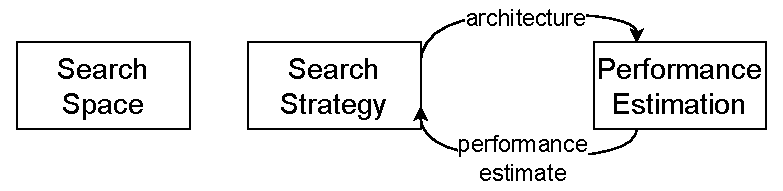
\includegraphics[scale=0.8, center]{graphics/nas.pdf}}
\end{figure}
\end{frame}
%- EfficientNet

\begin{frame}{Differentiable NAS}
\vspace{10pt}
\textit{DARTS} \cite{Liu2018} considered as pioneer work
\vfill
\begin{columns}
\begin{column}{.35\textwidth}
\begin{figure}
	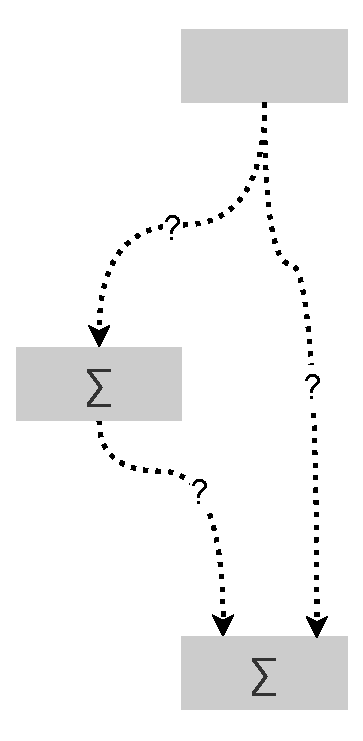
\includegraphics[scale=0.4, center]{graphics/darts_0.pdf}
\end{figure}
\end{column}
\begin{column}{.3\textwidth}
\end{column}
\begin{column}{.35\textwidth}
\end{column}
\end{columns}
\end{frame}

\begin{frame}{Differentiable NAS}
\vspace{10pt}
\textit{DARTS} \cite{Liu2018} considered as pioneer work
\vfill
\begin{columns}
\begin{column}{.35\textwidth}
\begin{figure}
	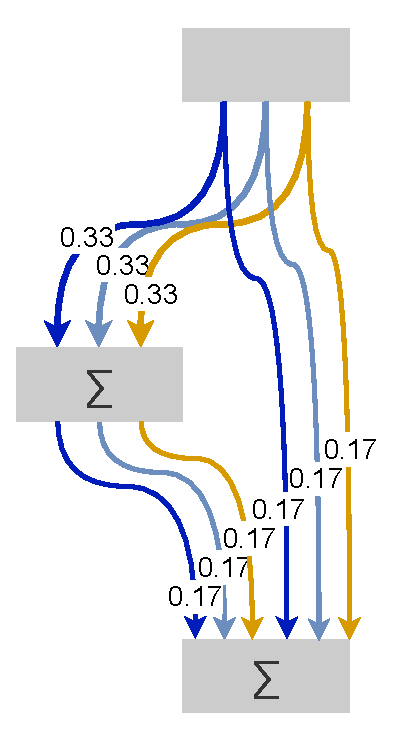
\includegraphics[scale=0.4, center]{graphics/darts_1.pdf}
\end{figure}
\end{column}
\begin{column}{.3\textwidth}
\end{column}
\begin{column}{.35\textwidth}
\end{column}
\end{columns}
\end{frame}

\begin{frame}{DARTS}
\vspace{10pt}
\textit{DARTS} \cite{Liu2018} considered as pioneer work
\vfill
\begin{columns}
\begin{column}{.35\textwidth}
\begin{figure}
	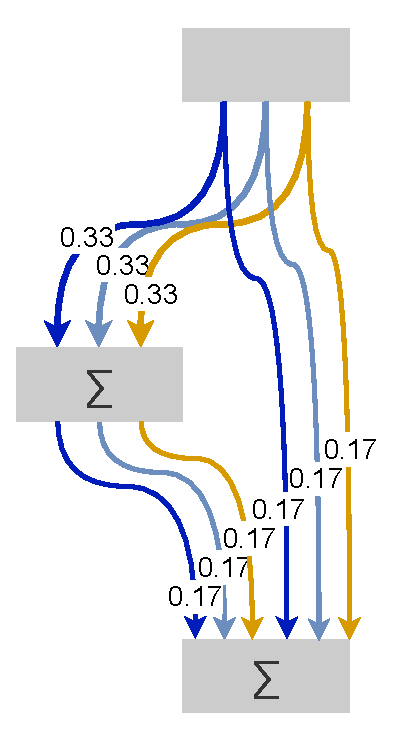
\includegraphics[scale=0.4, center]{graphics/darts_1.pdf}
	\caption{Training start}
\end{figure}
\end{column}
\begin{column}{.3\textwidth}
\begin{figure}
	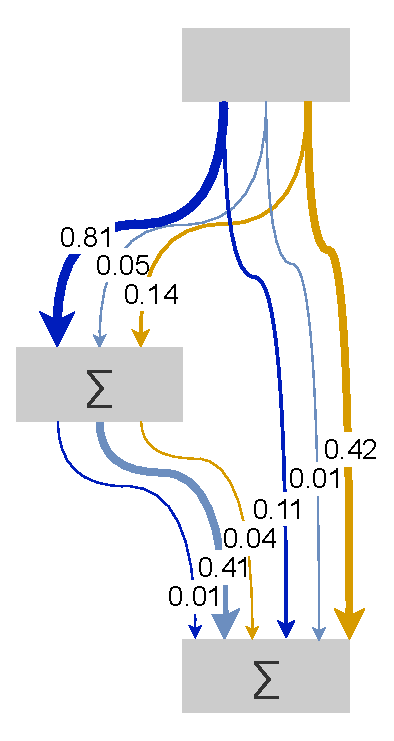
\includegraphics[scale=0.4, center]{graphics/darts_2.pdf}
	\caption{Training end}
\end{figure}
\end{column}
\begin{column}{.35\textwidth}
\begin{figure}
	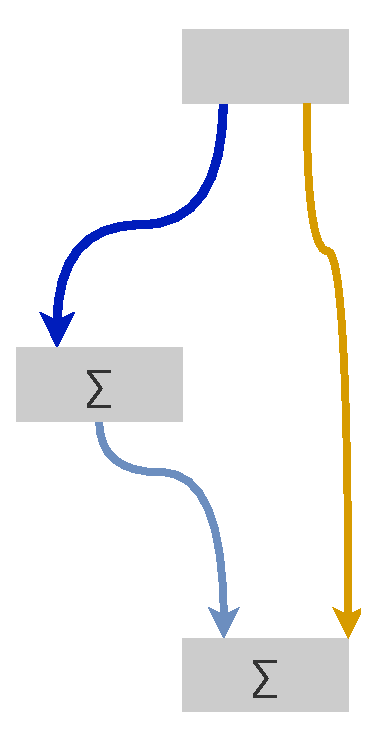
\includegraphics[scale=0.4, center]{graphics/darts_3.pdf}
	\caption{Obtain best architecture}
\end{figure}
\end{column}
\end{columns}
\end{frame}
%- "NASNet search space"
%- aggregation function
%	- logits versus Softmax
%	- weighted Sum vs. Multinomial sampling
%- success factors:
%	- Bi-Level optimization:
%		- different versions
%		- first-order version similar to coordinate descent, though on distinct datasets
%	- Zoph search space

\begin{frame}{Gumbel-Softmax Sampling}
\vspace{10pt}
We define the \textit{Standard Gumbel} probability density as
\begin{equation*}
g:\mathbb{R}\rightarrow [0,1],x\mapsto \exp^{-(x+\exp^{-x})}
\end{equation*}
For $k\in\mathbb{N}, G\sim P^k_g$ and architecture parameters $a\in\mathbb{R}^k$ it holds:
\begin{equation*}
\text{Softmax}(a + G, 0)\sim \text{Multinomial}(1, \text{Softmax}(a))
\end{equation*}
\end{frame}
%differentiablity maintained by approximating temperature 0 arbitrarily close

\section{DARTS as Surrogate}
\begin{frame}{Search Space}
\vspace{5pt}
\vfill
\begin{figure}
    \begin{center}
    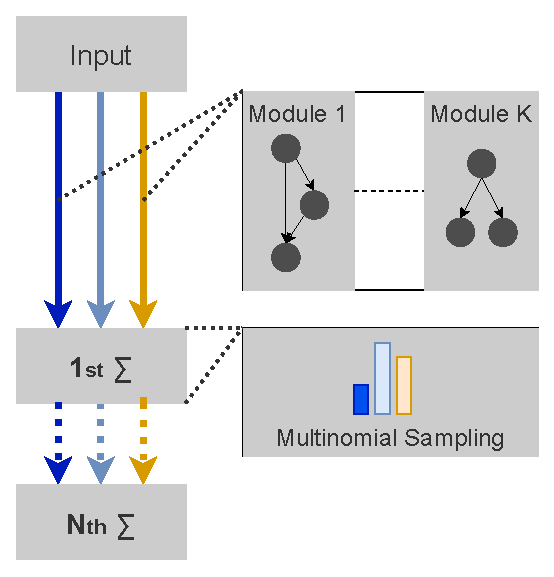
\includegraphics[scale=.75]{graphics/v3_search_space.pdf}
    \caption{}
  \end{center} 
\end{figure}
\end{frame}
%- distinctions to DARTS:
%	- Macro level and thus entire search space (as opposed to single cell)
%	- Gumbel Softmax
%- notion of cell

\begin{frame}{Relative Surrogate}
\vspace{10pt}
Joint trained multinomials induce ranking on search space
\vfill
\begin{figure}
    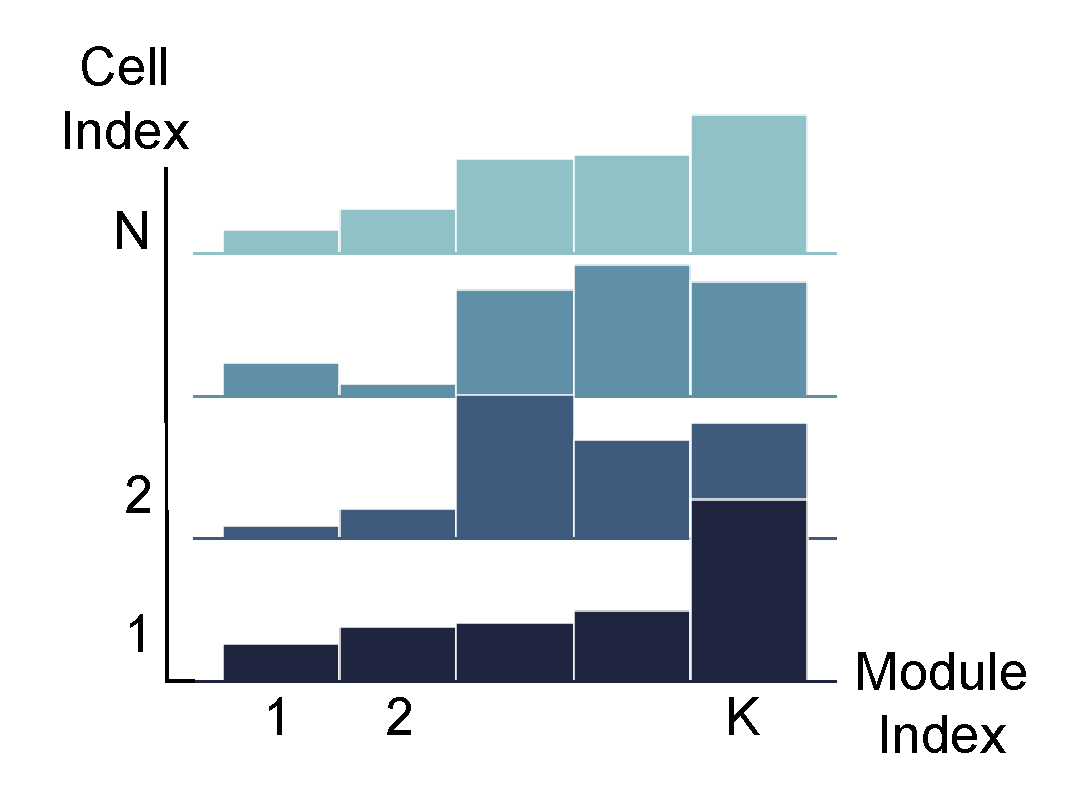
\includegraphics[scale=0.38, center]{graphics/v2_marginals.pdf}
    \caption{Sampling probability per module per cell}
\end{figure}
\end{frame}
%- independence assumption allows exponential search in linear cost

\begin{frame}{Relative Surrogate}
\vspace{10pt}
Validate surrogate ranking on actual architecture performances
\vfill
\begin{figure}
    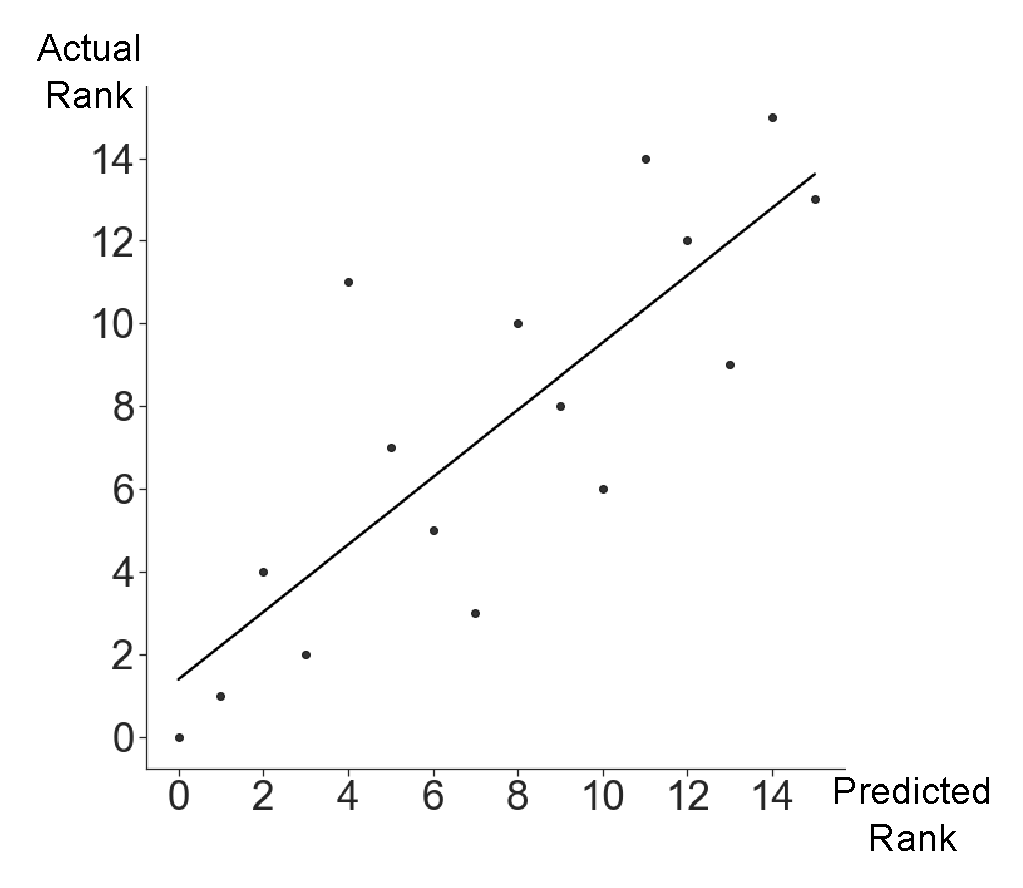
\includegraphics[scale=0.45, center]{graphics/spearman_validation.pdf}
\end{figure}
\end{frame}
%- sample random architecture test set on a space that will LATER be introduced
%- ablation studies

\begin{frame}{Architecture Regularization}
\vspace{10pt}
Control speed of convergence dependent on cell index
\vfill
\begin{figure}
    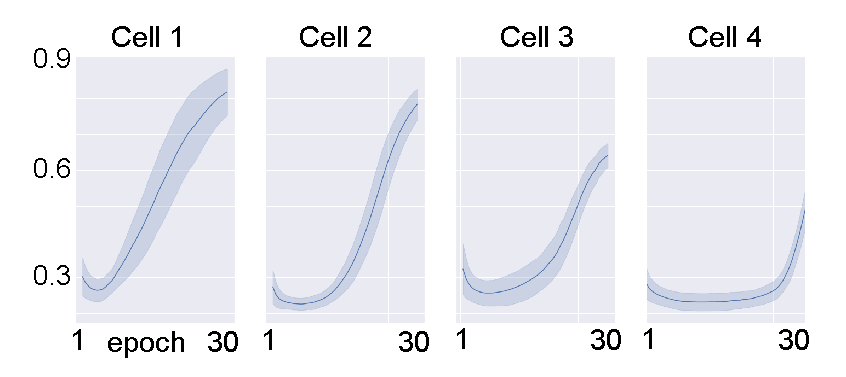
\includegraphics[scale=0.75, center]{graphics/alpha_curves.pdf}
    \caption{Maximum norm of architecture parameter vector per epoch per cell}
\end{figure}
\end{frame}
%- ~example for ablation study

\section{Beyond Finite Search Spaces}
\begin{frame}{Search Space Extension}
\vspace{10pt}
\vfill
\begin{figure}
    \begin{center}
    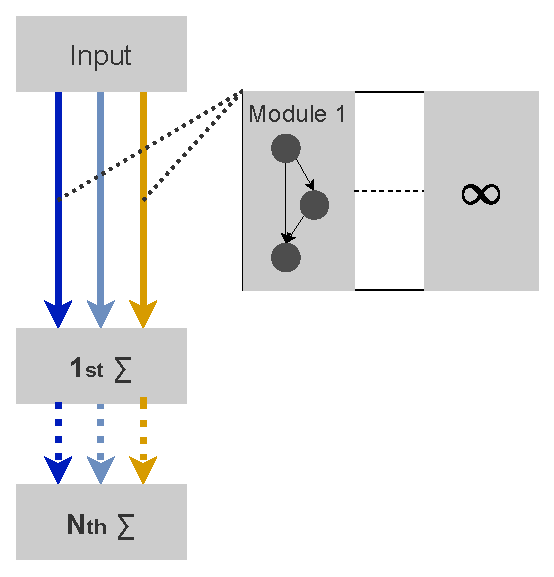
\includegraphics[scale=0.75]{graphics/search_space_extension.pdf}
    \caption{}
  \end{center} 
\end{figure}
\end{frame}

\begin{frame}{Finite Difference Descent}
\vspace{10pt}
Finite difference descent on pseudo environment in euclidean search space
\vspace{10pt}
\vfill
\begin{figure}
\begin{center}
\begin{overprint}
\onslide<1>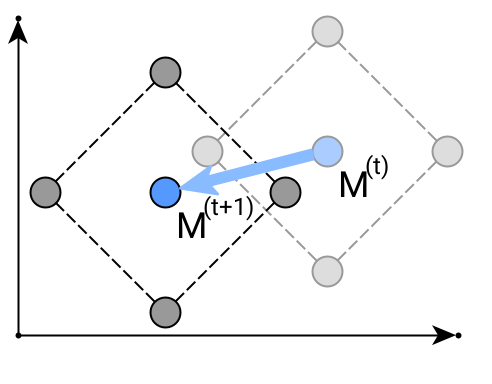
\includegraphics[scale=0.32, center]{graphics/v2_window.png}
\caption{2-dim euclidean search space}
%\onslide<2>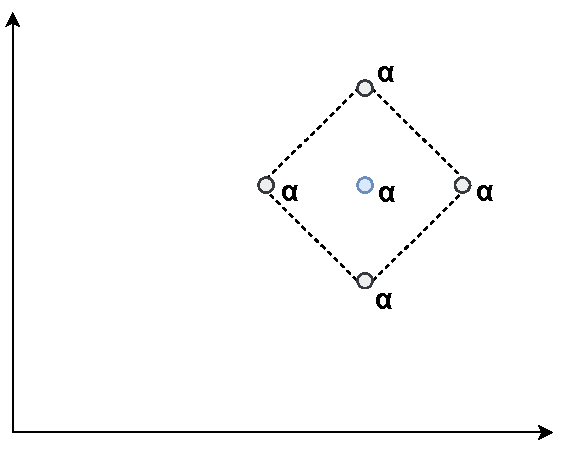
\includegraphics[scale=0.65, center]{graphics/window2.pdf}
%\caption{Euclidean search space}
%\onslide<3>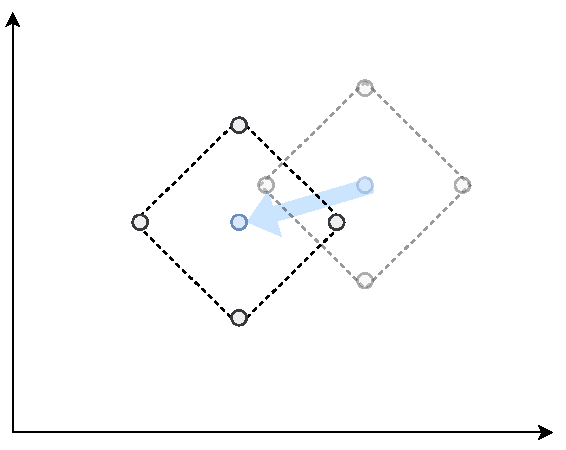
\includegraphics[scale=0.65, center]{graphics/window3.pdf}
%\caption{Euclidean search space}
\end{overprint}
\end{center}
\end{figure}
\end{frame}

\begin{frame}{Experimental Search Space}
\vspace{10pt}
We model architectures with directed acyclic graphs (DAG)
\vfill
\begin{figure}
\visible<2>{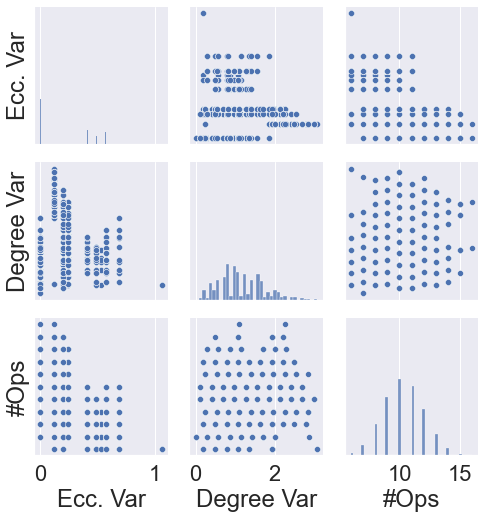
\includegraphics[scale=0.28, center]{graphics/experiments_search_space.png}}
\visible<2>{\caption{Eccentricity variance, degree variance and \# edges for 6-vertice DAGs}}
\end{figure}
\end{frame}

\begin{frame}{Experiment Results}
\vspace{10pt}
Search space trajectories (per dimension) for one exemplary cell over $100$ epochs of finite difference descent
\vspace{10pt}
\vfill
\begin{figure}
    \begin{center}
    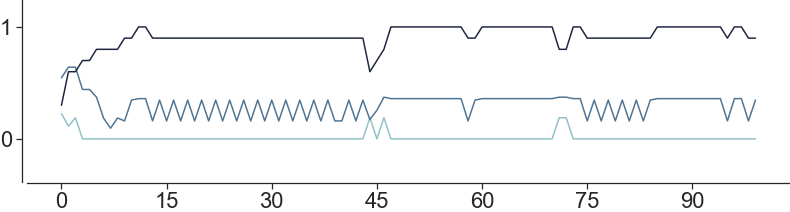
\includegraphics[scale=.7]{graphics/traject_f2_cell1.png}
  \end{center}
\end{figure}
\end{frame}

\begin{frame}{Experiment Results}
\vspace{10pt}
Comparing performance of top $10$ architectures found by Random Search, Bayesian Search and our approach
\vfill
\begin{figure}
    \begin{center}
    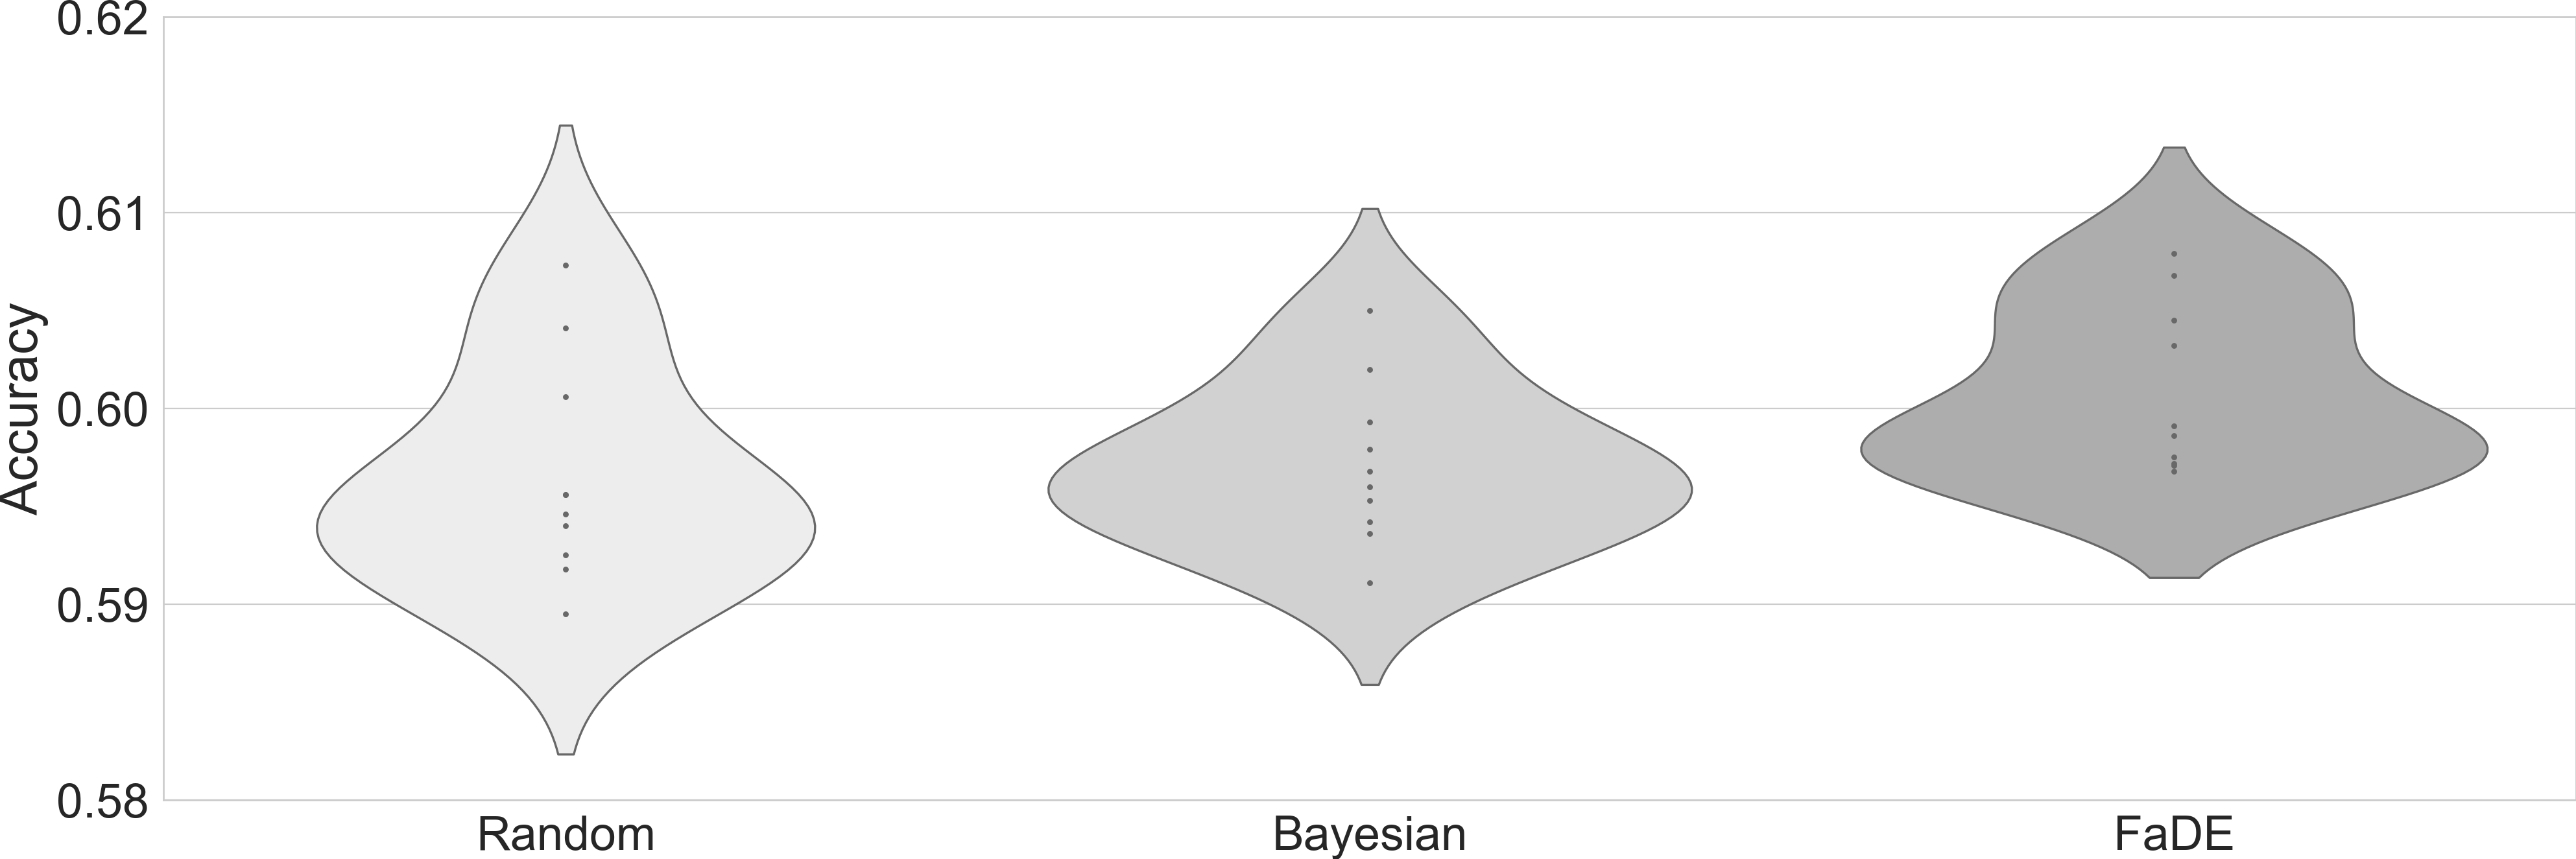
\includegraphics[scale=.22]{graphics/benchmark.png}
    \caption{}
  \end{center} 
\end{figure}
\end{frame}

\miniframesoff
\begin{frame}{References}
\bibliographystyle{apalike}
\bibliography{bib}
\end{frame}

\miniframeson
\end{document}
